\documentclass[nofilelist]{cslthse-msc}
% to show a list of used packages at the end of the document, delete the nofilelist option
%\documentclass{cslthse-msc}
\usepackage[utf8]{inputenc}
\usepackage[main=british,swedish]{babel}
\usepackage{amsmath}
%\usepackage{amsfonts}
%%\usepackage{amssymb}
\usepackage{amsthm}
%\usepackage{makeidx}
\usepackage{graphicx}
\usepackage[titletoc, header, page]{appendix}
\usepackage{transparent}
\usepackage{tikz}
\usepackage{enumitem}
\usepackage{listings}
\usepackage{svg}
\usepackage{subcaption}
\usetikzlibrary{fit,positioning,shapes.geometric}

\lstdefinestyle{mystyle}{
  basicstyle=\ttfamily\footnotesize,
  breakatwhitespace=false,
  breaklines=true,
  captionpos=b,
  keepspaces=true,
  numbers=left,
  numbersep=5pt,
  showspaces=false,
  showstringspaces=false,
  showtabs=false,
  tabsize=2
}
\lstset{style=mystyle}
\lstdefinelanguage{jrag}[]{java}{
  morekeywords={aspect, syn, eq, inh}
}
\begin{document}
\begin{equation}
  \tag{T-If}
  \frac{
    t_1 : \text{Bool}\quad
    t_2 : \text{T}\quad
    t_3 : \text{T}
  }{
    \text{if } t_1 \text{ then } t_2 \text{ else } t_3 : \text{T}
  }
\end{equation}



  \resizebox{\textwidth}{!}{%
  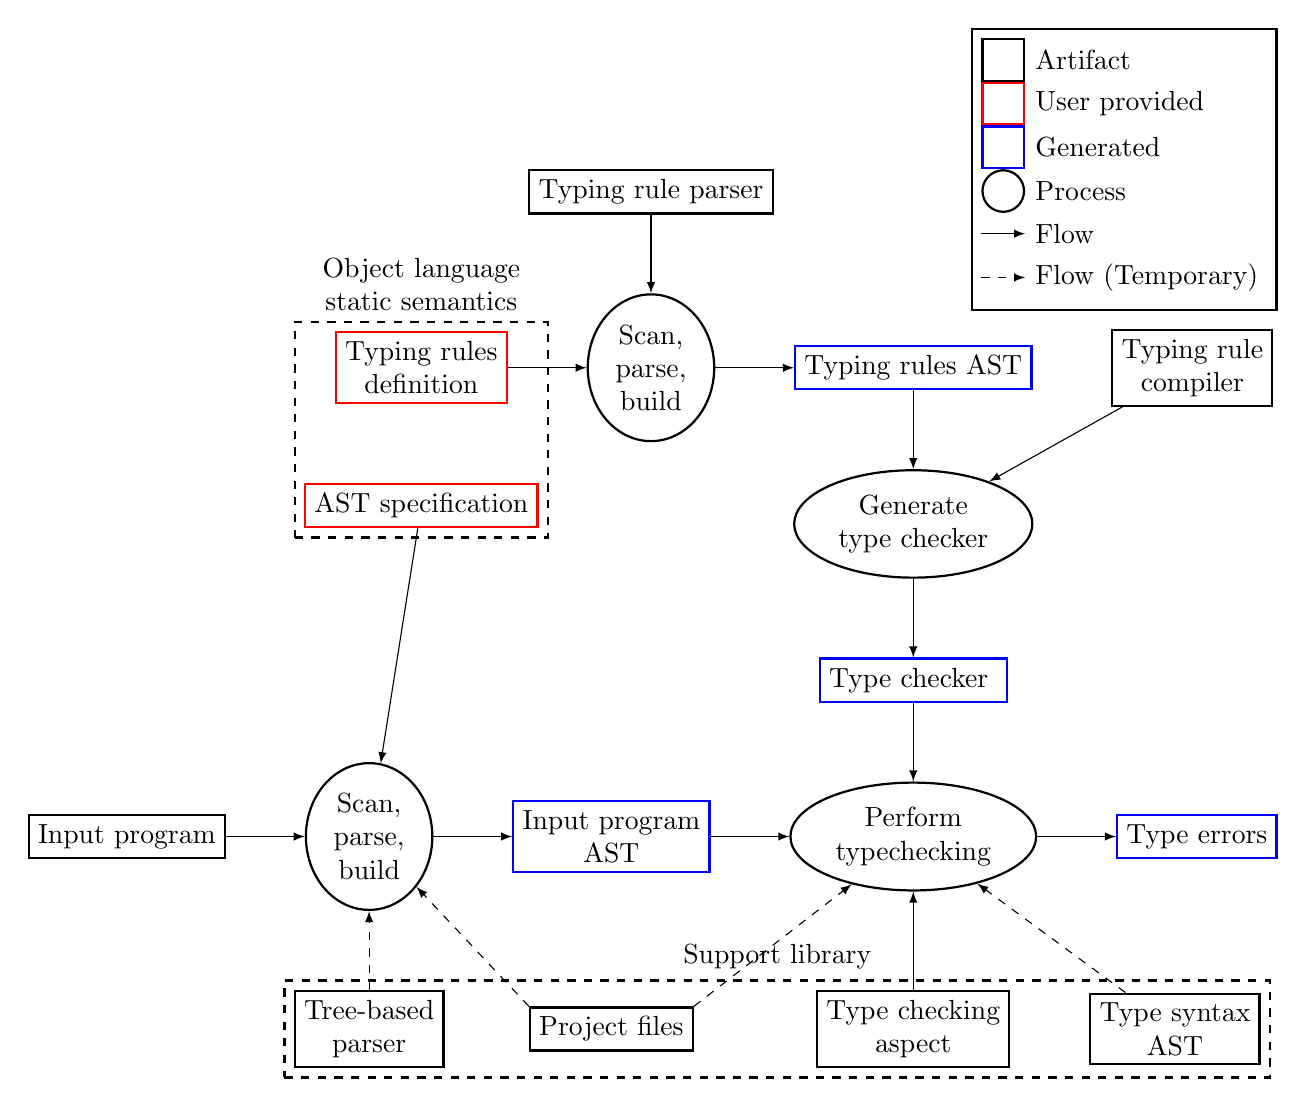
\begin{tikzpicture}[
      every node/.style = {align=center, line width=0.8pt},
      every path/.style = {draw, -latex},
      artifact/.style={draw=black},
      userinput/.style={draw=red},
      generated/.style={draw=blue},
      process/.style={ellipse, draw=black}
      %greennode/.style={shape=circle, draw=green, line width=2},
      %rednode/.style={shape=circle, draw=red, line width=2}
    ]
    \node (typerules) [userinput]                    {Typing rules\\definition };
    \node (trparsing) [right=of typerules, process] {Scan,\\parse,\\build};
    \node (trparser)  [above=of trparsing, artifact]          {Typing rule parser};
    \node (trast)     [right=of trparsing, generated]          {Typing rules AST};

    %\node (typecheckgen) [below=of trast, process, text width=5cm] {
    %  \textbf{Type checker generation}\\
    %  \hrule
    %  \begin{itemize}[noitemsep,topsep=2pt]
    %    \item Copy template
    %    \item Generate type checker from typing rules
    %  \end{itemize}
    %};
    \node (typecheckgen)       [below=of trast, process] {Generate\\type checker};
    \node (typingrulecompiler) [right=of trast, artifact]          {Typing rule\\compiler };
    \node (typechecker)        [below=of typecheckgen, generated]   {Type checker };

    \node (olast)     [below=of typerules, userinput] {AST specification};

    \node (outputtypechecking) [below=of typechecker, process] {Perform\\typechecking};
    \node (inputast)           [left=of outputtypechecking, generated]    {Input program\\AST};
    \node (outputparsing)      [left=of inputast, process]     {Scan,\\parse,\\build};
    \node (typeerrors)         [right=of outputtypechecking, generated]   {Type errors};
    \node (inputprog)          [left=of outputparsing, artifact]         {Input program};

    %\node (template) [below=of inputast, text width=6cm] {
    %  \textbf{Type checker template}\\
    %  \hrule
    %  \begin{itemize}[noitemsep,topsep=2pt]
    %    \item Scanner, parser, builder
    %    \item Project files
    %    \item Type checking algorithm 
    %  \end{itemize}
    %};
    \node (templateparser)        [below=of outputparsing, artifact]                               {Tree-based\\parser};
    \node (templateprojectfiles)  at (inputast |- templateparser)           [artifact]           {Project files};
    \node (typecheckingalgorithm) at (outputtypechecking |- templateparser) [artifact]           {Type checking\\aspect };
    \node (templatetypesyntax)    [right=of typecheckingalgorithm, artifact]                       {Type syntax\\AST };
    \node (template)              [dashed, fit=(templateparser) (typecheckingalgorithm) (templatetypesyntax), artifact] {};
    \node                         [above, draw=none] at (template.north)                 {Support library};

    \node (userinput)   [dashed, fill=none, fit=(typerules) (olast), artifact]                  {};
    \node               [above, draw=none] at (userinput.north)                       {Object language\\static semantics};
    %\node (typechecker) [dashed, fill=none, fit=(outputparsing) (outputtypechecking)] {};
    %\node               [above, draw=none] at (typechecker.north)                     {Type checker};

    \draw (typerules)          to (trparsing);
    \draw (trparser)           to (trparsing);
    \draw (trparsing)          to (trast);
    \draw (trast)              to (typecheckgen);
    \draw (typingrulecompiler) to (typecheckgen);
    \draw (typechecker)        to (outputtypechecking);
    \draw (olast)              to (outputparsing);
    \draw (outputparsing)      to (inputast);
    \draw (inputast)           to (outputtypechecking);
    \draw (outputtypechecking) to (typeerrors);
    \draw (typecheckgen)       to (typechecker);
    \draw (inputprog)          to (outputparsing);

    \draw[dashed] (templateparser)                  to (outputparsing);
    \draw         (typecheckingalgorithm)           to (outputtypechecking);
    \draw[dashed] (templateprojectfiles.north west) to (outputparsing);
    \draw[dashed] (templateprojectfiles.north east) to (outputtypechecking);
    \draw[dashed] (templatetypesyntax)              to (outputtypechecking);

    \matrix [left, nodes={minimum size = 15pt, align=left}, align=left, draw=black] at (current bounding box.north east) {
      \node [artifact, label=right:Artifact] {}; \\
      \node [userinput, label=right:User provided] {}; \\
      \node [generated, label=right:Generated] {}; \\
      \node [process, label=right:Process] {}; \\
      \node [draw=none, label=right:Flow] (leg1){}; \\
      \node [draw=none, label=right:Flow (Temporary)] (leg2){}; \\
    };
    \draw [label=right:Line] (leg1.west) to (leg1.east);\\
    \draw [dashed, label=right:Dashed] (leg2.west) to (leg2.east);\\

  \end{tikzpicture}
  }

\pagebreak
\begin{lstlisting}[language=jrag]
aspect TypingRules {

  syn Type True.type() {
    return new Bool();
  }

  syn Type False.type() {
    return new Bool();
  }
  syn Type Zero.type() {
    return new Int();
  }

  syn Type Or.type() {
    ASTNode left = getChild(0);
    ASTNode right = getChild(1);

    if(left.type().matches(new Bool()) &&
       right.type().matches(new Bool())) {
      return new Bool();
    }
    throw new RuntimeException("Typechecking failed");
  }
}
\end{lstlisting}

\begin{lstlisting}[]
[T-True]
True : Bool

[T-False]
False : Bool

[T-Zero]
Zero : Int

[T-Or]
left : Bool,
right : Bool
----------------------
Or(left, right) : Bool
\end{lstlisting}

\begin{lstlisting}[]
[T-True]
True : Bool

[T-False]
False : Bool

[T-Zero]
Zero : Int

[T-Or]
left : Bool,
right : Bool
----------------------
Or(left, right) : Bool
\end{lstlisting}

\pagebreak
\begin{lstlisting}[language=jrag, linewidth=350pt]
syn Type If.type() {
  ASTNode x = getChild(0);
  ASTNode y = getChild(1);
  ASTNode z = getChild(2);

  Type tyvar_a = null;
  if(tyvar_a == null)
    tyvar_a = y.type();
  else if (!tyvar_a.matches(y.type()))
    throw new RuntimeException("Typechecking failed: Type variable mismatch");
  if(tyvar_a == null)
    tyvar_a = z.type();
  else if (!tyvar_a.matches(z.type()))
    throw new RuntimeException("Typechecking failed: Type variable mismatch");
  if(x.type().matches(new Bool()) &&
     y.type().matches(tyvar_a) &&
     z.type().matches(tyvar_a)) {
    return tyvar_a;
  }
  throw new RuntimeException("Typechecking failed");
}
\end{lstlisting}
\end{document}
